\documentclass[10pt,twocolumn]{article}

\usepackage[margin=1in]{geometry}
\usepackage{amsmath,amssymb}
\usepackage{booktabs}
\usepackage{graphicx}
\usepackage{pgfplots}
\pgfplotsset{compat=1.18}
\usepackage{tikz}
\usetikzlibrary{arrows.meta,positioning,shapes.geometric,fit,calc,decorations.pathreplacing}
\usepackage{hyperref}
\usepackage[numbers]{natbib}
\usepackage{xcolor}
\usepackage{enumitem}
\usepackage[expansion=false]{microtype}
\usepackage{caption}
\usepackage{multirow}
\usepackage{siunitx}
\usepackage{pifont}

\setlength{\columnsep}{0.25in}
\emergencystretch=1em

% Color palette (extended from Paper 1)
\definecolor{cfresh}{HTML}{2196F3}
\definecolor{cfull}{HTML}{4CAF50}
\definecolor{ctargeted}{HTML}{FF9800}
\definecolor{cbaseline}{HTML}{9E9E9E}
\definecolor{cthorne}{HTML}{E91E63}
\definecolor{cvalid}{HTML}{4CAF50}
\definecolor{cinvalid}{HTML}{E91E63}
\definecolor{cva}{HTML}{FF9800}
\definecolor{cmean}{HTML}{2196F3}
\definecolor{ckinetic}{HTML}{E91E63}
\definecolor{cepistemic}{HTML}{9C27B0}
\definecolor{cstrict}{HTML}{2196F3}
\definecolor{crelaxed}{HTML}{FF5722}

\title{Continuous Control and Structural Regularization\\in Multi-Agent Narrative Extraction}
\author{
  Jack Chaudier Gaffney\\
  \texttt{jackchaudier@gmail.com}
}
\date{}

\begin{document}
\maketitle

% ============================================================
% ABSTRACT
% ============================================================
\begin{abstract}
A companion paper demonstrated that coordinated goal evolution restores arc quality in deterministic multi-agent narrative simulations suffering from chain degradation. Here we subject that finding to population-level analysis across 50 seeds and 3,250 deterministic simulation runs, revealing a quality-validity tradeoff: full evolution maximizes raw arc quality (mean~$Q = 0.684$) but destabilizes structural extraction, dropping the all-valid rate from 88\% to 64\%. We introduce a continuous interpolation parameter~$\alpha$ that blends default and evolved goal profiles, identifying an optimal operating point ($\alpha = 0.5$ for the agent whose evolution most destabilizes extraction) that preserves 95\% extraction validity while retaining the quality gains. A factorial decomposition shows that evolution is primarily a repair mechanism as measured by validity-adjusted score, while still providing modest quality amplification in fresh environments. Investigating why extraction fails, we find that the strict beat grammar acts as a structural regularizer: relaxing it collapses performance because the search exploits loosened constraints. A detailed case study of a peripheral agent reveals premature turning-point anchoring as the specific failure mechanism---the extraction search locks onto an early high-tension event, and the grammar's monotonic phase rule permanently closes the development phase. Brute-force feasibility analysis shows that 96.8\% of mid-arc events, when forced as turning points with optimized surrounding-event selection, yield at least one structurally valid arc construction, establishing that the grammar provides a coherence floor rather than a meaning discriminator. Tracing the mechanism further, we show that a single sequential constraint (\texttt{min\_development\_beats}) is a necessary condition for 100\% of observed extraction failures---all invalid arcs lack development beats---while the other three constraint dimensions have zero or marginal effect, and that the search's candidate pools are entirely degenerate: importance-driven protagonist-event injection---structurally necessary for peripheral agents---contaminates every pool with early catastrophes. A temporal filter on the injection set recovers 7 of 9 focal failures. All experiments are fully deterministic at \$0.00 compute cost.
\end{abstract}


% ============================================================
% 1. INTRODUCTION
% ============================================================
\section{Introduction}
\label{sec:intro}

Gaffney~\cite{gaffney2026goal} demonstrated that multi-agent narrative simulations with persistent world state suffer from \emph{chain degradation}: as secrets resolve and beliefs saturate across sequential episodes, agents with fixed goals produce declining arc quality. Coordinated goal evolution across all six agents closed 89\% of the quality gap on a single seed, revealing a collective threshold effect where partial evolution is counterproductive.

That analysis had three limitations. First, the evolution experiment used a single seed (seed~7), leaving open whether the effect generalizes. Second, validity---whether the extraction pipeline can produce structurally legal arcs for all six agents simultaneously---was not analyzed: the single seed happened to yield six valid arcs under all conditions. Third, the \emph{mechanism} by which evolution interacts with extraction was not investigated.

This paper addresses all three. We scale to 50~seeds and 3,250~deterministic runs, revealing a quality-validity tradeoff that was invisible at single-seed resolution. We introduce continuous control over evolution intensity, characterize the strict beat grammar as a structural regularizer, and trace a specific failure mode---premature turning-point anchoring leading to phase collapse---through a sequence of diagnostic experiments that progressively narrow the hypothesis space.

Our contributions are:
\begin{enumerate}[nosep]
\item A population-level analysis showing that chain degradation is real but weaker and more heterogeneous than single-seed estimates suggested (gap of 0.007 vs.\ 0.053), and that coalition composition dominates coalition size in determining quality outcomes.
\item Continuous $\alpha$-interpolation between default and evolved goal profiles, revealing a Pareto-optimal operating point where validity is preserved while quality gains are retained.
\item A factorial decomposition establishing that evolution is primarily a repair mechanism for information-depleted environments as measured by validity-adjusted score, while still modestly amplifying mean quality in fresh environments.
\item Experimental evidence that the strict beat grammar acts as a structural regularizer: relaxing grammar constraints during search collapses extraction performance, even though the relaxed validator is a true superset of the strict one.
\item A complete mechanistic account of extraction failure: premature turning-point anchoring traced to candidate pool contamination via importance-driven event injection, with base-rate feasibility analysis (96.8\% grammar saturation) and a temporal filtering fix that recovers 7/9 focal seeds.
\end{enumerate}

All experiments are fully deterministic and reproducible from fixed random seeds at \$0.00 compute cost per condition.\footnote{Seeds 1--50 for population experiments. 20-seed subsets for $\alpha$-sweeps. Scripts and output data available upon request.}


% ============================================================
% 2. RELATED WORK
% ============================================================
\section{Related Work}
\label{sec:related}

We extend the related work survey in~\cite{gaffney2026goal} with three additional threads relevant to this paper's findings.

\paragraph{Narrative extraction as constrained optimization.}
Story sifting~\cite{garbe2019storysifting} and its successors~\cite{kreminski2020winnow,kreminski2022loose} retrieve narrative patterns from simulation logs but do not frame extraction as an optimization problem with explicit quality objectives. Curation-oriented work in simulated storyworlds similarly emphasizes retrieval and authoring interfaces over formal objective analysis~\cite{ryan2018curveship}. Our Rashomon extraction optimizes a composite $Q$-metric subject to beat grammar constraints, making it amenable to analysis through the lens of constrained optimization and regularization.

\paragraph{Goodhart's law in generative systems.}
When a measure becomes a target, it ceases to be a good measure~\cite{goodhart1984problems}. In reinforcement learning, reward hacking occurs when agents exploit proxy objectives in unintended ways~\cite{amodei2016concrete,skalse2022defining}. Our finding that relaxing grammar constraints enables the search to exploit the $Q$-metric---selecting incoherent high-tension fragments---is a structural analog: the grammar acts as a regularizer preventing metric exploitation, much as constraints in RL prevent reward hacking.

\paragraph{Quality-diversity in procedural generation.}
MAP-Elites~\cite{mouret2015illuminating}, novelty search~\cite{lehman2011abandoning}, and procedural content generation surveys~\cite{gravina2019procedural,risi2020increasing} motivate search strategies that preserve behavioral diversity rather than collapsing to a single greedy optimum. Our identification of two failure regimes---search exploration failure (where better valid arcs exist but are not found) and metric misalignment (where the metric genuinely prefers invalid arcs)---suggests that quality-diversity search over turning-point positions could address the first regime without architectural changes.


% ============================================================
% 3. SYSTEM DESCRIPTION
% ============================================================
\section{System Description}
\label{sec:system}

We use the \textsc{NarrativeField} pipeline described in~\cite{gaffney2026goal}: deterministic simulation of six agents across five locations (${\sim}200$ events per run), a seven-dimension composite $Q$-metric (Eq.~2 in~\cite{gaffney2026goal}), and Rashomon extraction producing one arc per agent with beat grammar validation. We introduce three additions.

\paragraph{Validity-adjusted score.}
The $Q$-metric scores individual arcs but does not penalize a system that produces high-quality arcs for some agents while failing to produce valid arcs for others. We define the validity-adjusted score as:
\begin{equation}
\label{eq:va}
\text{VA} = \frac{1}{N} \sum_{s=1}^{N} \bar{Q}_s \times \frac{v_s}{6}
\end{equation}
where $\bar{Q}_s$ is the mean $Q$-score across the $v_s$ \emph{valid} arcs in seed~$s$ (invalid arcs are excluded from the average, not scored as zero), $v_s$ is the number of agents with structurally valid arcs, and $N$ is the total number of seeds (where the summand evaluates to 0 when $v_s = 0$, i.e., seeds with no valid arcs contribute zero to VA). The $v_s/6$ term penalizes seeds with fewer valid arcs, while $\bar{Q}_s$ reflects the quality of arcs that the extractor successfully produced. Seeds with partial validity degrade gracefully rather than being zeroed out. VA captures both quality and extraction feasibility in a single number.
We separately report the \emph{all-valid rate}, $n_{\text{all-valid}} / N$, the fraction of seeds where all six agents produce structurally valid arcs. This is a stricter binary measure: a seed contributes to the all-valid rate only if all six arcs pass validation.

\paragraph{Alpha interpolation.}
To treat evolution intensity as a continuous control parameter, we introduce $\alpha \in [0,1]$ per agent, interpolating between default goals ($\alpha = 0$) and fully-evolved goals ($\alpha = 1$):
\begin{equation}
\label{eq:alpha}
\theta(\alpha) = (1 - \alpha)\,\theta_{\text{default}} + \alpha\,\theta_{\text{evolved}}
\end{equation}
where $\theta$ denotes the full agent parameter vector (goal dimensions, closeness values, relationship triples). This applies independently to each scalar field; categorical fields (commitments) use the evolved value when $\alpha \geq 0.5$ and the default otherwise.

\paragraph{Beat grammar recap.}
Each extracted arc must contain $\geq$1 \textsc{setup} beat, $\geq$1 development beat (\textsc{complication} or \textsc{escalation}), exactly~1 \textsc{turning\_point}, and $\geq$1 \textsc{consequence}. Phase progression must be monotonic (setup $\to$ development $\to$ crisis $\to$ resolution; no reversals). The protagonist must appear in $\geq$60\% of arc events, and consecutive events must share causal links. Additionally, arcs must contain between 4 and 20 beats and span at least 15\% of total simulation time (with an absolute floor of 10~sim minutes). These constraints are unchanged from~\cite{gaffney2026goal}.

\paragraph{Extraction search.}
Event importance is the event's precomputed significance metric when available; otherwise a composite of event-type weight (ranging from 5.0 for \textsc{catastrophe} to 0.3 for \textsc{social\_move}) plus half the delta signal, which sums the count and magnitude of non-pacing state changes (beliefs, relationships, secret states).

The arc search selects up to eight high-importance anchor events from the protagonist's event window, then expands each anchor via BFS (depth~3) over the causal link graph to form a candidate event pool. Each pool is downsampled to at most 20 events preserving protagonist involvement and causal continuity, beats are classified and enforced into monotonic phase progression, and the resulting arc is validated against the grammar. The search returns the valid candidate with the highest composite $Q$-score. It does not backtrack: once an anchor is expanded and its candidate arc constructed, downstream beat assignments are fixed by the monotonic phase rule.


% ============================================================
% 4. POPULATION-LEVEL ANALYSIS
% ============================================================
\section{Population-Level Analysis}
\label{sec:population}

\subsection{Experimental Setup}

For each of seeds 1--50, we generate a depth-2 canon (stories $A \to B$), then run story~$C$ under multiple evolution conditions. At each coalition size $k \in \{0, \ldots, 6\}$, we test all $\binom{6}{k}$ coalition combinations, yielding $50 \times \sum_{k=0}^{6}\binom{6}{k} = 50 \times 64 = 3{,}200$ runs for the $k$-sweep plus 50 fresh (depth-0) baseline runs, totaling 3,250~runs. All runs are deterministic.

\subsection{Chain Degradation at Population Scale}

\begin{table}[t]
\centering
\caption{Key conditions across 50 seeds. Full evolution ($k{=}6$) maximizes mean $Q$ but minimizes VA due to validity collapse. Excl-Thorne ($k{=}5$) matches baseline validity while improving quality.}
\label{tab:ksweep}
\begin{tabular}{lcccc}
\toprule
\textbf{Condition} & \textbf{Mean $Q$} & \textbf{VA} & \textbf{All-Valid} \\
\midrule
Fresh (depth-0)       & 0.674 & 0.661 & 88\% \\
Baseline ($k{=}0$, D2) & 0.667 & 0.652 & 88\% \\
$k{=}6$ full evolution  & 0.684 & 0.623 & 64\% \\
$k{=}5$ excl-Thorne    & 0.686 & 0.661 & 88\% \\
\bottomrule
\end{tabular}
\end{table}

Table~\ref{tab:ksweep} reports the key conditions. At population scale, chain degradation is real but small: the depth-0 fresh mean is 0.674 versus depth-2 baseline 0.667, a gap of 0.007---substantially smaller than the single-seed gap of 0.053 reported in~\cite{gaffney2026goal}. The effect is heterogeneous: 31/50~seeds show degradation under canon accumulation while 19/50~show improvement, confirming that degradation is a population tendency rather than a universal law.

\subsection{The Quality-Validity Tradeoff}

\begin{figure}[t]
\centering
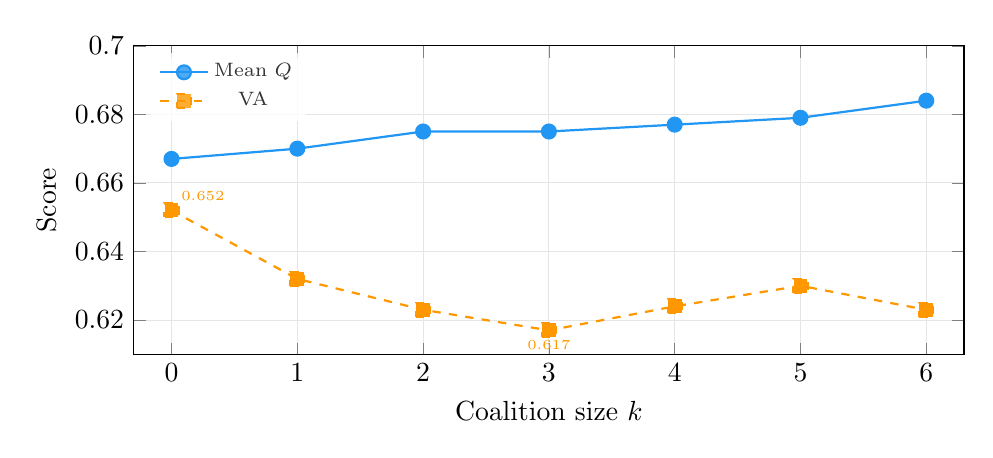
\begin{tikzpicture}
\begin{axis}[
  width=\columnwidth,
  height=5.5cm,
  xlabel={Coalition size $k$},
  ylabel={Score},
  xmin=-0.3, xmax=6.3,
  ymin=0.61, ymax=0.70,
  xtick={0,1,2,3,4,5,6},
  ytick={0.62,0.64,0.66,0.68,0.70},
  grid=major,
  grid style={gray!20},
  legend style={at={(0.02,0.98)}, anchor=north west, font=\scriptsize, draw=none, fill=white, fill opacity=0.8},
  every axis plot/.append style={mark size=2.5pt, thick},
]
\addplot[cmean, mark=*, solid]
  coordinates {(0,0.667)(1,0.670)(2,0.675)(3,0.675)(4,0.677)(5,0.679)(6,0.684)};
\addplot[cva, mark=square*, dashed]
  coordinates {(0,0.652)(1,0.632)(2,0.623)(3,0.617)(4,0.624)(5,0.630)(6,0.623)};
\node[font=\tiny, cva, anchor=south west] at (axis cs:0,0.652) {0.652};
\node[font=\tiny, cva, anchor=north] at (axis cs:3,0.617) {0.617};
\legend{Mean $Q$, VA}
\end{axis}
\end{tikzpicture}
\caption{Mean $Q$ and VA score by coalition size $k$. Mean $Q$ increases monotonically with $k$. VA declines from $k{=}0$ to a minimum at $k{=}3$, partially recovers at $k{=}4$--$5$, and drops again at $k{=}6$ as the all-valid rate falls from 88\% to 64\%.}
\label{fig:ksweep}
\end{figure}

Figure~\ref{fig:ksweep} reveals the central tension of this paper. Mean $Q$ increases monotonically with coalition size $k$, peaking at $k{=}6$ (0.684). VA declines from $k{=}0$ (0.652) to a minimum at $k{=}3$ (0.617), partially recovers at $k{=}4$--$5$ as coalition composition effects favor validity-preserving combinations, then drops again at $k{=}6$ (0.623). The quality-validity tradeoff is not a simple endpoint collapse but operates throughout the coalition size range, with mid-range coalitions producing the worst validity-adjusted outcomes. The all-valid rate and VA tell complementary stories: the binary all-valid rate collapses at the endpoint ($k{=}6$, 64\% vs.\ 88\% at $k{=}0$), while the continuous VA measure reveals that partial validity erosion begins at $k{=}1$ and is worst at $k{=}3$.

At $k{=}6$, per-agent validity rates range from Diana (82\%) and Thorne (88\%) to Marcus (100\%), with Elena at 90\%, Victor at 92\%, and Lydia at 94\%. Diana's disproportionate failure rate motivates the detailed diagnostic in Section~\ref{sec:collapse}.

\subsection{Composition Outweighs Size}

Within-$k$ variance is $2$--$3\times$ larger than between-$k$ improvement: at $k{=}1$, the variance across the six single-agent coalitions (0.00269) exceeds the mean improvement from $k{=}0$ to $k{=}1$ (0.003). Shapley value analysis across all coalitions ranks Elena as the highest-leverage single target ($+0.009$) and Diana as the only negative contributor ($-0.005$). Excluding Elena from a $k{=}5$ coalition is catastrophic: quality drops below $k{=}3$ levels. These results confirm and extend the ``Elena as canary'' finding from~\cite{gaffney2026goal}: Elena's goal--world misalignment (secrecy goals when the affair is universally known) is the single largest driver of degradation.

\subsection{Genre Shift}

\begin{table}[t]
\centering
\caption{Mean event counts by condition and their shift from baseline ($k{=}0$) to full evolution ($k{=}6$) across 50 seeds. Evolution drives a robust genre shift toward surveillance and conflict.}
\label{tab:genre}
\begin{tabular}{lrrr}
\toprule
\textbf{Event Type} & \textbf{Baseline} & \textbf{Full Evol.} & \textbf{$\Delta$} \\
\midrule
observe     & 48.4 & 60.6 & $+$12.2 \\
conflict    & 7.5 & 11.3 & $+$3.8 \\
catastrophe & 2.7 & 7.4 & $+$4.7 \\
chat        & 22.7 & 11.9 & $-$10.8 \\
\bottomrule
\end{tabular}
\end{table}

The genre shift reported in~\cite{gaffney2026goal} for a single seed replicates robustly at population scale (Table~\ref{tab:genre}). Evolution shifts the event distribution from social chatter toward surveillance and conflict, with \textsc{observe} events increasing by $+12.2$ and \textsc{chat} decreasing by $-10.8$ on average. This shift is independent of extraction validity---it occurs in both valid and invalid runs.


% ============================================================
% 5. CONTINUOUS CONTROL
% ============================================================
\section{Continuous Control}
\label{sec:continuous}

\subsection{Alpha-Sweep}

\begin{figure}[t]
\centering
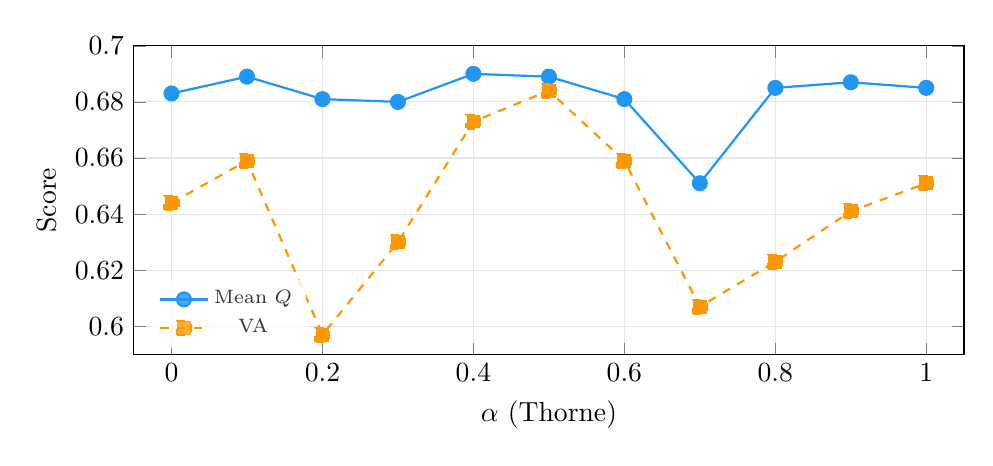
\begin{tikzpicture}
\begin{axis}[
  width=\columnwidth,
  height=5.5cm,
  xlabel={$\alpha$ (Thorne)},
  ylabel={Score},
  xmin=-0.05, xmax=1.05,
  ymin=0.59, ymax=0.70,
  xtick={0,0.2,0.4,0.6,0.8,1.0},
  ytick={0.60,0.62,0.64,0.66,0.68,0.70},
  grid=major,
  grid style={gray!20},
  legend style={at={(0.02,0.02)}, anchor=south west, font=\scriptsize, draw=none, fill=white, fill opacity=0.8},
  every axis plot/.append style={mark size=2.5pt, thick},
]
\addplot[cmean, mark=*, solid]
  coordinates {(0,0.683)(0.1,0.689)(0.2,0.681)(0.3,0.680)(0.4,0.690)(0.5,0.689)(0.6,0.681)(0.7,0.651)(0.8,0.685)(0.9,0.687)(1.0,0.685)};
\addplot[cva, mark=square*, dashed]
  coordinates {(0,0.644)(0.1,0.659)(0.2,0.597)(0.3,0.630)(0.4,0.673)(0.5,0.684)(0.6,0.659)(0.7,0.607)(0.8,0.623)(0.9,0.641)(1.0,0.651)};
\legend{Mean $Q$, VA}
\end{axis}
\end{tikzpicture}
\caption{Thorne $\alpha$-sweep (20 seeds, all other agents at $\alpha{=}1.0$). Mean $Q$ is approximately flat across $\alpha$, but VA is sharply peaked at $\alpha{=}0.5$ (0.684, 95\% all-valid). The optimum is driven entirely by validity preservation, not raw quality. Point-to-point VA variation reflects the 20-seed sample size; the $\alpha{=}0.5$ peak is corroborated by the coordinate descent result in Section~\ref{sec:continuous}.}
\label{fig:alpha_curve}
\end{figure}

The $k$-sweep showed that full evolution ($k{=}6$) maximizes mean $Q$ but minimizes VA. Can evolution intensity be treated as a continuous control parameter? We sweep $\alpha \in \{0.0, 0.1, \ldots, 1.0\}$ for Thorne (with all other agents at $\alpha = 1.0$) across 20~seeds ($20 \times 11 = 220$ runs).

Figure~\ref{fig:alpha_curve} shows the result. Mean $Q$ varies only between 0.651 and 0.690 across the $\alpha$ range---effectively flat. But VA is sharply peaked at $\alpha = 0.5$ (VA $= 0.684$, 95\% all-valid). The optimum is driven entirely by validity preservation: $\alpha = 0.5$ reduces the intensity of Thorne's evolved profile (e.g., \texttt{truth\_seeking} interpolated to 0.775 instead of 0.95), keeping the simulation in a regime where extraction succeeds for peripheral agents. We note that $\alpha = 0.5$ is exactly the boundary where the interpolation rule (Eq.~\ref{eq:alpha}) switches categorical commitment fields from default to evolved. The validity spike at this point therefore reflects continuous goal parameters at half intensity \emph{combined with} the first adoption of Thorne's evolved categorical commitments. These two effects---dampened continuous goals stabilizing extraction versus the categorical toggle potentially destabilizing it---may partially offset, and disentangling their individual contributions is left for future work.

\subsection{Coordinate Descent}

Optimizing $\alpha$ per-agent via coordinate descent yields a final vector: Thorne~0.5, Elena~1.0, Marcus~1.0, Lydia~1.0, Diana~0.25, Victor~1.0. The pattern is interpretable: agents whose evolved profiles destabilize extraction (Thorne, Diana) receive reduced intensity; agents whose evolution is universally beneficial (Elena, Marcus, Lydia, Victor) remain at full intensity.

However, this optimized vector does not significantly outperform simpler heuristics at 50-seed scale (Table~\ref{tab:references}). The optimal $\alpha$ condition and the excl-Thorne $k{=}5$ condition produce statistically indistinguishable VA scores ($z \approx 0.26$, $p > 0.7$).

\begin{table}[t]
\centering
\caption{Reference conditions at 50-seed scale. The optimal $\alpha$-vector and excl-Thorne $k{=}5$ are statistically indistinguishable; both substantially outperform full evolution on VA.}
\label{tab:references}
\begin{tabular}{lccc}
\toprule
\textbf{Condition} & \textbf{Mean $Q$} & \textbf{VA} & \textbf{Valid} \\
\midrule
Optimal $\alpha$     & 0.683 & 0.665 & 88\% \\
Excl-Thorne ($k{=}5$) & 0.686 & 0.661 & 88\% \\
Full evolution ($k{=}6$) & 0.684 & 0.623 & 64\% \\
Baseline ($k{=}0$)   & 0.667 & 0.652 & 88\% \\
\bottomrule
\end{tabular}
\end{table}

\subsection{Factorial Decomposition}

\begin{table}[t]
\centering
\caption{Factorial design: 2 depths (D0 fresh, D2 degraded) $\times$ 3 evolution levels (default, evolved=$\alpha$-optimal, full=$\alpha{=}1.0$). The same evolved profiles \emph{help} validity at D2 (88\%) but \emph{hurt} at D0 (76\%).}
\label{tab:factorial}
\begin{tabular}{lccc}
\toprule
\textbf{Condition} & \textbf{Mean $Q$} & \textbf{VA} & \textbf{Valid} \\
\midrule
D0-default  & 0.674 & 0.661 & 88\% \\
D0-evolved  & 0.682 & 0.633 & 76\% \\
D0-full     & 0.694 & 0.635 & 68\% \\
\midrule
D2-default  & 0.667 & 0.652 & 88\% \\
D2-evolved  & 0.683 & 0.665 & 88\% \\
D2-full     & 0.684 & 0.623 & 64\% \\
\bottomrule
\end{tabular}
\end{table}

To isolate the causal effects of evolution, we run a $2 \times 3$ factorial design: two depths (D0 fresh, D2 degraded) crossed with three evolution levels (default, evolved=$\alpha$-optimal, full=$\alpha = 1.0$ all agents). Table~\ref{tab:factorial} reports the results (50~seeds each, 300~runs total).

The key interaction: the same evolved profiles that maintain 88\% validity at D2 drop to 76\% at D0. Evolution is not a generic amplifier---it is primarily a repair mechanism for information-depleted environments as measured by VA. Decomposing the effects:

\begin{itemize}[nosep]
\item \textbf{Amplifier effect} (D0: default$\to$evolved): $+0.008$ mean, $-0.028$ VA. Evolution improves raw quality in fresh environments but hurts extractability.
\item \textbf{Degradation effect} (D0$\to$D2, default): $-0.007$ mean, $-0.009$ VA. Weak baseline degradation.
\item \textbf{Repair effect} (D2: default$\to$evolved): $+0.016$ mean, $+0.013$ VA. Evolution at D2 improves both quality \emph{and} validity.
\end{itemize}

The repair effect exceeds the amplifier effect by 4~VA points. On mean $Q$, both D0 and D2 still improve under evolved profiles. The depleted canon provides structural scaffolding that constrains agent behavior into extractable patterns; evolution works \emph{with} this scaffolding at D2 but \emph{against} it at D0.


% ============================================================
% 6. GRAMMAR AS STRUCTURAL REGULARIZER
% ============================================================
\section{Grammar as Regularizer}
\label{sec:grammar}

\subsection{Grammar Relaxation}

If the strict beat grammar (exactly~1 turning point, 0 phase regressions) is too rigid, relaxing it should recover invalid arcs. We test a relaxed grammar allowing 1--2 turning points and $\leq$1 phase regression, re-running extraction under both grammars across three conditions (50~seeds each, 150~runs total).

\begin{table}[t]
\centering
\caption{Grammar relaxation collapses extraction. The relaxed grammar is strictly more permissive but produces dramatically worse all-valid rates across all conditions.}
\label{tab:relaxation}
\begin{tabular}{lcccc}
\toprule
 & \multicolumn{2}{c}{\textbf{Strict}} & \multicolumn{2}{c}{\textbf{Relaxed}} \\
\cmidrule(lr){2-3} \cmidrule(lr){4-5}
\textbf{Condition} & \textbf{VA} & \textbf{Valid} & \textbf{VA} & \textbf{Valid} \\
\midrule
Baseline      & 0.652 & 88\% & 0.542 & 32\% \\
Full evolution & 0.623 & 64\% & 0.530 & 36\% \\
Excl-Thorne   & 0.661 & 88\% & 0.490 & 24\% \\
\bottomrule
\end{tabular}
\end{table}

Table~\ref{tab:relaxation} shows that relaxation makes everything worse. Baseline all-valid drops from 88\% to 32\%; excl-Thorne drops from 88\% to 24\%. The relaxed grammar is strictly more permissive as a \emph{validator}, but when used during \emph{search}, the expanded candidate space allows the $Q$-metric to select incoherent high-tension fragments that happened to satisfy the looser constraints. At the per-agent level, Diana recovers completely under relaxed search (9 invalid $\to$ 0), but Marcus goes from 0 to 19 invalid arcs---the search trades one agent's coherence for another's.

\subsection{Constraint Dimensionality}
\label{sec:constraint_dim}

Which grammar constraints carry the regularization effect? We sweep each of the grammar's four constraint dimensions independently, relaxing one at a time while holding the others strict, across 50~seeds under full evolution.

\begin{table}[t]
\centering
\caption{Single-dimension constraint relaxation under full evolution (50~seeds). Only \texttt{min\_development\_beats} produces a measurable effect on the all-valid rate; the other three dimensions are structurally inert.}
\label{tab:constraint_dim}
\scriptsize
\begin{tabular}{lcc}
\toprule
\textbf{Dimension relaxed} & \textbf{All-Valid} & \textbf{$\Delta$ from strict} \\
\midrule
None (strict baseline) & 64\% & --- \\
\texttt{min\_development\_beats} ($1 \to 0$) & 100\% & $+$36pp \\
\texttt{max\_phase\_regressions} ($0 \to 999$) & 70\% & $+$6pp \\
\texttt{protagonist\_coverage} ($0.60 \to 0.0$) & 64\% & 0pp \\
\texttt{min\_timespan\_fraction} ($0.15 \to 0.0$) & 64\% & 0pp \\
\bottomrule
\end{tabular}
\end{table}

Table~\ref{tab:constraint_dim} shows that a single \emph{sequential} structural constraint is a necessary condition for 100\% of observed extraction failures: requiring at least one development beat before the turning point. All invalid arcs across the failing seeds lack development beats; the other three constraint dimensions have zero or marginal effect (Table~\ref{tab:constraint_dim}). Removing the development-beat requirement raises the all-valid rate from 64\% to 100\%---every arc becomes valid when development beats are optional. The other three constraint dimensions (phase regression tolerance, protagonist coverage, minimum timespan) have zero or marginal effect. The grammar's regularization is not volumetric (broadly shrinking the feasible set) but sequential: it requires a specific ordering property---development before crisis---that the search's greedy importance-driven selection systematically violates for peripheral agents.

\subsection{Depth Invariance}
\label{sec:depth_invariance}

Is the regularization cliff an artifact of information-depleted environments, or does it reflect a search-algorithmic property? We repeat the \texttt{min\_development\_beats} sweep at depth-0 (fresh, no canon) and depth-2 (degraded).

\begin{table}[t]
\centering
\caption{Development-beat constraint cliff at two canon depths (50~seeds each, full evolution). The cliff magnitude is within 5 percentage points across depths.}
\label{tab:depth_invariance}
\scriptsize
\begin{tabular}{lcc}
\toprule
\textbf{min\_dev\_beats} & \textbf{D0 All-Valid} & \textbf{D2 All-Valid} \\
\midrule
0 & 100\% & 100\% \\
1 & 68\% & 64\% \\
\midrule
Cliff ($\Delta$) & 32pp & 36pp \\
\bottomrule
\end{tabular}
\end{table}

The 0$\to$1 cliff appears at both depths with nearly identical magnitude (Table~\ref{tab:depth_invariance}): 32~percentage points at depth-0 versus 36 at depth-2. The mechanism is search-algorithmic---the search's importance-driven pool construction produces the same turning-point anchoring failure regardless of whether the simulation environment is fresh or information-depleted.

\subsection{Rescore-Only Test}
\label{sec:rescore}

Is the collapse caused by the relaxed validator or the relaxed search? We perform a decisive experiment: take all arcs extracted under the \emph{strict} grammar and re-validate them using the \emph{relaxed} validator, without re-running the search.

\begin{table}[t]
\centering
\caption{Rescore-only results. Strict-valid arcs remain relaxed-valid (the relaxed grammar is a true superset). But zero strict-invalid arcs recover---the arcs fail for content reasons, not constraint reasons.}
\label{tab:rescore}
\scriptsize
\begin{tabular}{lc}
\toprule
\textbf{Test} & \textbf{Result} \\
\midrule
Strict-valid $\to$ relaxed-valid & 855/855 (100\%) \\
Strict-invalid $\to$ recovered & 0/45 (0\%) \\
\midrule
\multicolumn{2}{l}{\textbf{Invalid arc failure reasons (45 arcs):}} \\
\midrule
Missing \textsc{complication} or \textsc{escalation} & 42/45 (93\%) \\
Causal continuity violation & 3/45 (7\%) \\
Phase monotonicity violation & 0/45 (0\%) \\
Turning-point count violation & 0/45 (0\%) \\
\bottomrule
\end{tabular}
\end{table}

Table~\ref{tab:rescore} is definitive. All 855 strict-valid arcs pass the relaxed validator (confirming the relaxed grammar is a true superset). But 0/45 strict-invalid arcs recover---the invalid arcs fail because they lack development beats entirely (42/45) or violate causal continuity (3/45), neither of which is addressed by allowing additional turning points or phase regressions. The failure mode is content absence---the arcs lack development-phase events entirely---not constraint mismatch, where correct content exists in the wrong structural configuration. No grammar relaxation can recover content that was never selected.

The grammar constraints play a dual role: they define structural validity \emph{and} act as an inductive bias that regularizes the extraction search against metric exploitation. Relaxing constraints during candidate generation (not just validation) collapses performance because the search exploits loosened constraints to select incoherent high-tension fragments. The strict grammar is a structural regularizer, not a measurement bottleneck.

\subsection{Validity Covariance}

Is extraction validity zero-sum across agents---does one agent's valid arc come at the expense of another's? Across all 3,250 $k$-sweep runs, we compute pairwise validity correlations. No negative correlations appear in the aggregate matrix; the strongest correlation is Thorne--Lydia at $+0.435$. Marcus is never invalid at $k{=}6$ (entire column null). Mean $Q$ by valid-arc count declines modestly: 0.680 for 6-valid seeds, 0.675 for 5-valid, 0.665 for 4-valid. Validity and quality are aligned, not in tension. Validity is a collective property: when one agent's arc goes invalid, it does not free narrative resources for others.


% ============================================================
% 7. ANATOMY OF PHASE COLLAPSE
% ============================================================
\section{Anatomy of Phase Collapse}
\label{sec:collapse}

Under full evolution, Diana (an evader/observer) produces 9/50 invalid arcs, all failing for the identical reason: ``Missing \textsc{complication} or \textsc{escalation} beat.'' We conduct a series of diagnostic experiments to identify the mechanism.

\subsection{Event Composition}

\begin{table}[t]
\centering
\caption{Diana valid vs.\ invalid arcs under full evolution. Invalid arcs have equal involvement and arc length but zero development beats and 16.4 \textsc{consequence} beats (vs.\ 7.8 in valid arcs).}
\label{tab:diana}
\scriptsize
\begin{tabular}{p{0.42\columnwidth}cc}
\toprule
\textbf{Metric} & \textbf{Valid ($N{=}41$)} & \textbf{Invalid ($N{=}9$)} \\
\midrule
Sim involvement & 43.5 & 42.7 \\
Arc events & 20.0 & 20.0 \\
\textsc{complication} beats & 3.3 & 0.0 \\
\textsc{escalation} beats & 2.9 & 0.0 \\
\textsc{consequence} beats & 7.8 & 16.4 \\
\midrule
TP position (mean) & 0.66 & 0.12 \\
TP position (median) & 0.69 & 0.13 \\
Events before TP & 11.2 & 2.6 \\
Events after TP & 7.8 & 16.4 \\
\bottomrule
\end{tabular}
\end{table}

Table~\ref{tab:diana} shows that Diana is not event-starved: her invalid arcs draw from 42.7 simulation events on average, exceeding Thorne's 35.6. Both valid and invalid arcs contain exactly 20 arc events. The difference is entirely structural: invalid arcs contain 0.0 \textsc{complication} and 0.0 \textsc{escalation} beats, with 16.4 \textsc{consequence} beats consuming the arc. For comparison, Marcus (46.6 mean involvement, 100\% valid under full evolution) never fails.

\subsection{Temporal Distribution}

Diana's invalid arcs are not temporally skewed. The late share ($>$0.70 in simulation time) is 33.3\% for invalid arcs versus 35.7\% for valid, and the mean global position of her events is 0.49 (invalid) versus 0.53 (valid). Events are spread across the full timeline. The \textsc{complication} and \textsc{escalation} beat counts are 0 in all temporal segments (early, mid, late)---mid-timeline events that should be labeled as development are instead being labeled \textsc{consequence}.

\subsection{Turning-Point Anchoring}

\begin{figure}[t]
\centering
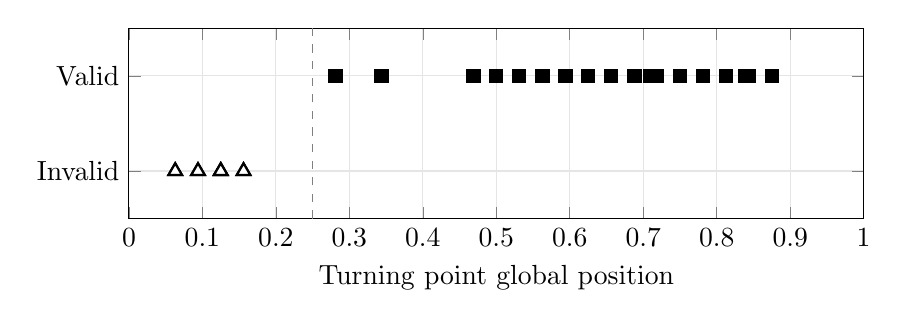
\begin{tikzpicture}
\begin{axis}[
  width=0.9\columnwidth,
  height=4cm,
  xlabel={Turning point global position},
  ylabel={},
  xmin=0, xmax=1,
  ymin=0.5, ymax=2.5,
  ytick={1,2},
  yticklabels={Invalid, Valid},
  grid=major,
  grid style={gray!20},
  scatter/classes={
    valid={mark=square*,draw=black,fill=black,mark size=2.2pt,line width=0.8pt},
    invalid={mark=triangle*,draw=black,fill=white,mark size=2.8pt,line width=0.8pt}
  },
]
% Valid arcs - strip at y=2
\addplot[scatter, only marks, scatter src=explicit symbolic]
  coordinates {
    (0.625,2) [valid] (0.719,2) [valid] (0.844,2) [valid]
    (0.688,2) [valid] (0.839,2) [valid] (0.710,2) [valid]
    (0.839,2) [valid] (0.688,2) [valid] (0.625,2) [valid]
    (0.344,2) [valid] (0.563,2) [valid] (0.750,2) [valid]
    (0.500,2) [valid] (0.281,2) [valid] (0.656,2) [valid]
    (0.688,2) [valid] (0.750,2) [valid] (0.719,2) [valid]
    (0.813,2) [valid] (0.594,2) [valid] (0.719,2) [valid]
    (0.710,2) [valid] (0.656,2) [valid] (0.710,2) [valid]
    (0.875,2) [valid] (0.750,2) [valid] (0.531,2) [valid]
    (0.531,2) [valid] (0.656,2) [valid] (0.750,2) [valid]
    (0.344,2) [valid] (0.469,2) [valid] (0.750,2) [valid]
    (0.500,2) [valid] (0.875,2) [valid] (0.688,2) [valid]
    (0.839,2) [valid] (0.813,2) [valid] (0.563,2) [valid]
    (0.813,2) [valid] (0.781,2) [valid] (0.625,2) [valid]
  };
% Invalid arcs - strip at y=1
\addplot[scatter, only marks, scatter src=explicit symbolic]
  coordinates {
    (0.063,1) [invalid] (0.063,1) [invalid] (0.156,1) [invalid]
    (0.125,1) [invalid] (0.125,1) [invalid] (0.125,1) [invalid]
    (0.094,1) [invalid] (0.156,1) [invalid] (0.094,1) [invalid]
  };
% Separation line
\draw[gray, dashed, thin] (axis cs:0.25,0.5) -- (axis cs:0.25,2.5);
\node[font=\tiny, text=gray, anchor=south] at (axis cs:0.25,2.5) {0.25};
\end{axis}
\end{tikzpicture}
\caption{Turning-point position strip plot for Diana's arcs under full evolution (upper band: valid, $N{=}41$; lower band: invalid, $N{=}9$). All invalid arcs place the TP before position 0.25, while valid arcs cluster around 0.66--0.69. The gap is categorical---no overlap exists.}
\label{fig:tp_strip}
\end{figure}

Figure~\ref{fig:tp_strip} is the central diagnostic. In valid Diana arcs, the turning point sits at median position 0.69 (classical mid-to-late placement). In all 9 invalid arcs, the turning point is anchored before position 0.25 (median 0.13, max 0.16). The separation is categorical: zero overlap between the two distributions.

This is the mechanism. The extraction search selects a high-tension early event---likely an A-plot explosion that Diana witnesses---as her turning point. Because the grammar enforces monotonic phase progression, this early anchor permanently closes the development phase: everything after the turning point must be \textsc{consequence}. The 16.4~events-after-TP matches exactly the 16.4~\textsc{consequence} beats from Table~\ref{tab:diana}---they are the same number, because phase monotonicity forces all post-TP events into falling action.

We term this \emph{premature turning-point anchoring}: the search's greedy selection of a globally high-tension early event as a peripheral agent's climax, followed by monotonic phase collapse of the remaining arc.

\subsection{Phase Prior Intervention}

Can we fix this by constraining turning-point placement? We add a validator filter rejecting candidate arcs where the TP falls outside $[0.25, 0.70]$.

\begin{table}[t]
\centering
\caption{Phase-prior intervention outcomes (50 seeds, full evolution). Constraining TP position causes broad regressions and does not heal Diana's 9 failing seeds.}
\label{tab:phaseprior}
\begin{tabular}{lcc}
\toprule
\textbf{Agent} & \textbf{Strict $\to$ Prior} & \textbf{$\Delta$ valid} \\
\midrule
Diana  & 41 $\to$ 21 & $-20$ (0/9 healed) \\
Thorne & 44 $\to$ 21 & $-23$ \\
Marcus & 50 $\to$ 25 & $-25$ \\
\bottomrule
\end{tabular}
\end{table}

The intervention heals 0/9 of Diana's invalid arcs while causing 23~Thorne regressions and 25~Marcus regressions. The filter rejects candidates post-hoc, but the search still generates the same candidates using the same heuristics. Many valid arcs legitimately have TPs outside $[0.25, 0.70]$---Thorne's TPs range up to 0.88. Imposing rigid classical pacing windows on a heterogeneous agent population destroys authentic structural variance without addressing the root cause. The temporal injection filter introduced in Section~\ref{sec:pool_contamination} achieves what this phase prior cannot: rather than rejecting candidates post-hoc (after the search has already committed to contaminated pools), it removes the early-event contaminants from the injection set before pool construction, addressing the root cause upstream of candidate generation.

\subsection{Mid-Arc Feasibility}

If premature anchoring is the problem, do valid mid-arc alternatives exist? For each of Diana's 9 invalid seeds, we brute-force every Diana event in $[0.25, 0.70]$ as the turning point, building 20-event arcs around each and validating with the strict grammar.

Each candidate event is tested with multiple surrounding-event constructions (varying the number of pre-TP and post-TP events); we mark a candidate as feasible if at least one construction passes strict validation. All 9/9~seeds have valid mid-arc alternatives. Of 166 mid-arc candidates tested, 147 (88.6\%) produce structurally valid arcs under this max-over-attempts procedure. Diana's mid-arc region is not barren---it contains abundant viable turning points that the search does not find.

\subsection{Base-Rate Feasibility}

\begin{table}[t]
\centering
\caption{Base-rate feasibility comparison using identical brute-force construction and max-over-attempts scoring for each candidate event.}
\label{tab:baserate}
\begin{tabular}{lcc}
\toprule
\textbf{Seed Group} & \textbf{Valid Arcs} & \textbf{Rate} \\
\midrule
Invalid seeds (9) & 147/166 & 88.6\% \\
Valid seeds (41) & 794/820 & 96.8\% \\
\bottomrule
\end{tabular}
\end{table}

To calibrate the 88.6\% feasibility rate, we run the same brute-force procedure on Diana's 41 \emph{valid} seeds. Table~\ref{tab:baserate} shows the result: 794/820 candidates produce valid arcs (96.8\%), with a per-seed median of 100\%. In this setting, the grammar validates nearly any mid-arc candidate event once that event is forced as TP and paired with optimized surrounding-event selection.

This is \emph{grammar saturation}: in an environment where every agent participates in ${\sim}200$ interconnected events, many event neighborhoods can be assembled into structurally legal setup $\to$ development $\to$ crisis $\to$ resolution arcs. The grammar provides a necessary coherence floor---without it, the search grabs incoherent fragments (Section~\ref{sec:rescore})---but it is insufficient as a quality discriminator. The 88.6\% vs.\ 96.8\% rates are within 10~percentage points; in this case study, the grammar is approximately equally permissive regardless of whether the seed's natural extraction succeeds or fails.

\subsection{Seed Autopsy}

\begin{table}[t]
\centering
\caption{Turning-point event types in 147 valid mid-arc Diana arcs. Epistemic types (60.5\% of valid TPs) score approximately 0.17 points lower than kinetic types, despite producing equally valid arcs.}
\label{tab:tptypes}
\begin{tabular}{lrcc}
\toprule
\textbf{TP Type} & \textbf{Count} & \textbf{Share} & \textbf{Mean $Q$} \\
\midrule
\textsc{social\_move} & 65 & 44.2\% & 0.547 \\
\textsc{chat} & 29 & 19.7\% & 0.535 \\
\textsc{physical} & 15 & 10.2\% & 0.609 \\
\textsc{internal} & 14 & 9.5\% & 0.487 \\
\textsc{catastrophe} & 11 & 7.5\% & 0.704 \\
\textsc{observe} & 10 & 6.8\% & 0.522 \\
\textsc{conflict} & 2 & 1.4\% & 0.703 \\
\textsc{reveal} & 1 & 0.7\% & 0.634 \\
\midrule
\emph{Epistemic} & 89 & 60.5\% & ${\sim}$0.54 \\
\emph{Kinetic} & 13 & 8.8\% & 0.703 \\
\bottomrule
\end{tabular}
\end{table}

Table~\ref{tab:tptypes} breaks down the 147 valid mid-arc turning points by event type. The majority (60.5\%) are quiet, epistemic events (\textsc{social\_move}, \textsc{observe}, \textsc{internal}), scoring ${\sim}0.54$ on average (weighted mean 0.536). Only 8.8\% are kinetic events (\textsc{catastrophe}, \textsc{conflict}), scoring 0.703. Both produce structurally valid arcs, but the $Q$-metric scores kinetic TPs by approximately 0.17~points higher.

\begin{table}[t]
\centering
\caption{Seed-level autopsy for Diana's 9 failing seeds: comparison sign between best valid mid-arc alternative and the search-selected invalid arc.}
\label{tab:seed_autopsy}
\begin{tabular}{lcc}
\toprule
\textbf{Seed} & \textbf{Sign} & \textbf{Regime} \\
\midrule
2  & $\leq 0$ & Metric \\
3  & $\leq 0$ & Metric \\
9  & $> 0$ & Search \\
25 & $> 0$ & Search \\
32 & $> 0$ & Search \\
33 & $\leq 0$ & Metric \\
35 & $> 0$ & Search \\
38 & $\leq 0$ & Metric \\
43 & $> 0$ & Search \\
\bottomrule
\end{tabular}
\end{table}
In Table~\ref{tab:seed_autopsy}, ``Search'' denotes search exploration failure and ``Metric'' denotes metric misalignment.

Comparing the search-selected invalid arcs against the best valid mid-arc alternatives across the 9~invalid seeds reveals two failure regimes:

\begin{itemize}[nosep]
\item \textbf{Regime~1 (5/9~seeds):} The best valid mid-arc alternative outscores the search-selected invalid arc. A later kinetic event exists in mid-arc that the search failed to find. This is \emph{search exploration failure}---better arcs exist but the greedy search does not reach them.
\item \textbf{Regime~2 (4/9~seeds):} The search-selected invalid arc outscores the best valid alternative by a margin of 0.098 on average. Mid-arc options are purely epistemic. The $Q$-metric genuinely prefers the kinetic early spike over a structurally valid quiet turning point. This is \emph{substantial metric misalignment}---not catastrophic Goodhart, but a significant and measurable kinetic bias.
\end{itemize}
The comparison in Table~\ref{tab:seed_autopsy} is methodologically asymmetric: the ``best valid'' value is a max over many valid candidates per seed, while the search-selected value is a single greedy output. This winner's-curse asymmetry biases toward finding larger valid alternatives, so we treat the 5/9 vs.\ 4/9 split as a case-study diagnostic rather than a population estimate. We note that this taxonomy is \emph{counterfactual}: it characterizes what would happen if an oracle presented these mid-arc alternatives to the scoring function. For the 5/9 search-failure seeds, the oracle's alternative outscores the search-selected arc---the metric would have chosen correctly given access. For the 4/9 metric-misalignment seeds, even the oracle's best valid alternative loses to the early-TP arc---the metric genuinely prefers the structurally invalid option. Section~\ref{sec:pool_contamination} will show that the oracle scenario is moot: the search never generates these alternatives in the first place.

\subsection{Candidate Pool Contamination}
\label{sec:pool_contamination}

The seed autopsy (Section~\ref{sec:collapse}) identified premature turning-point anchoring as the proximate mechanism and classified failure seeds into search exploration failure (5/9) and metric misalignment (4/9). We now trace the mechanism to its root cause in the search's candidate pool construction.

\paragraph{Pool degeneracy.}
Across Diana's 9 invalid seeds, the search evaluates only 33 candidate arcs total, and all 33 have zero development beats with turning-point positions between 0.062 and 0.161. Every candidate in every pool exhibits the same pathology. For comparison, a matched sample of 9 valid seeds produces 38 candidates, of which 36 (94.7\%) have at least one development beat. The failing seeds' candidate pools are entirely degenerate---the search has zero valid alternatives to evaluate, regardless of anchor selection strategy.

\paragraph{Injection mechanism.}
This degeneracy is not caused by anchor selection bias. Forcing all 8 search anchors into the mid-arc region (positions 0.30--0.70) produces identical failures: the same 9 seeds fail with byte-identical arc structures (0/9 fixed across three anchor diversification strategies). The mechanism is upstream of anchor selection. The extraction architecture injects each protagonist's highest-importance events into every candidate pool (\texttt{proto\_keep\_ids} in the search implementation) to ensure dramatic relevance. This injection is structurally necessary: removing it entirely produces 0/50 valid arcs for Diana, whose peripheral causal footprint is too sparse for BFS-only pool construction. However, for agents whose highest-tension events are early catastrophes witnessed from the A-plot, the injection guarantees that the beat classifier assigns the turning point to those early events in every pool, and the monotonic phase rule collapses the remainder into falling action. This is a \emph{dual-function mechanism}: the same protagonist-event injection that makes peripheral-agent arc construction possible also makes it vulnerable to early-event contamination.

\paragraph{Temporal filtering.}
Temporally filtering the injection set to exclude events before position 0.20 recovers 7 of the 9 focal seeds (47/50 valid overall), confirming that the contamination vector is specifically early-event injection rather than the injection mechanism itself. One previously valid seed regresses under the filter; the 2 remaining focal failures (seeds 32, 38) represent borderline cases where Diana's high-tension events in the post-0.20 range are insufficient for valid arc construction. The development beat constraint thus functions as an integrity filter that detects when the global tension metric assigns a structurally incoherent turning point for the agent's local narrative---catching at the grammar level a pool-construction failure that no tested search strategy can avoid.


% ============================================================
% 8. DISCUSSION
% ============================================================
\section{Discussion}
\label{sec:discussion}

\subsection{Grammar as Coherence Floor}

The base-rate feasibility analysis (96.8\% candidate validity under forced-TP, optimized-surroundings construction) establishes that in dense deterministic simulations, the strict beat grammar is a minimum coherence filter, not a quality discriminator. It provides a necessary floor: without it, the search grabs incoherent fragments (Table~\ref{tab:relaxation}). But it is insufficient: it validates a large fraction of candidates in a causally dense environment. The gap between ``structurally legal'' and ``narratively meaningful'' is where extraction fails.

\subsection{The Kinetic Bias}

The $Q$-metric's approximately 0.17-point scoring gap between kinetic turning points (0.703) and epistemic ones (weighted mean 0.536) is doing the actual structural work of distinguishing narratively substantive from narratively thin events. Both produce valid arcs; only one class is rewarded by the metric. This is not a bug in the metric per se---kinetic events \emph{do} produce larger world-state changes---but it creates a systematic disadvantage for agents whose narrative arcs are driven by observation, realization, and social maneuvering rather than confrontation.

\subsection{Evolution as Pacing Control}

The factorial decomposition (Section~\ref{sec:continuous}) shows that $\alpha$ controls the rate at which the A-plot consumes the simulation's dramatic budget. At $\alpha = 0.5$, Thorne's truth-seeking is interpolated to 0.775 instead of 0.95, producing less extreme early confrontations. This keeps the search from borrowing the A-plot's early detonation as peripheral agents' climaxes. $\alpha$ does not fix the extractor---it keeps the simulation in a regime where the extractor's limitations do not bind.

The critical interaction in the factorial design reinforces this interpretation: the same evolved profiles maintain 88\% validity at depth-2 (where depleted canon provides structural scaffolding) but drop to 76\% at depth-0 (where fresh environments leave agents unconstrained). Evolution is primarily a repair mechanism on VA that works \emph{with} the scaffolding provided by information depletion, while still modestly improving mean $Q$ at depth-0.

\subsection{Phase Collapse: Syntax vs.\ Semantics}

Premature turning-point anchoring reveals a structural mismatch between two components of the extraction pipeline. The grammar evaluates \emph{syntax}: local phase coherence (does setup precede development precede crisis?). The $Q$-metric evaluates \emph{semantics}: macroscopic world-state changes (how much tension did the turning point generate?). When these diverge---when a syntactically legal arc is semantically thin, or a semantically rich event falls in the wrong syntactic position---extraction fails.

For Diana's invalid arcs, the metric correctly identifies the early A-plot explosion as the highest-tension event accessible to her arc. The grammar correctly rejects the resulting arc for lacking development. Neither component is wrong in isolation; the failure is in their interaction, mediated by a search that optimizes the metric without visibility into the grammar's downstream requirements. The pool contamination analysis (Section~\ref{sec:pool_contamination}) traces this interaction further: the search's candidate pools are entirely degenerate (0/33 valid candidates) because importance-driven event injection guarantees early catastrophes enter every pool. This injection is structurally necessary for peripheral agents---without it, Diana produces 0/50 valid arcs---so the grammar's role extends beyond detecting syntax/semantics mismatch to detecting pool-level contamination that no tested search strategy can avoid.

\subsection{Implications}

These findings suggest a general tension that may arise in any multi-protagonist extraction architecture that combines a greedy quality metric with structural grammar constraints. The core problem---that a shared event timeline viewed through a fixed grammar template cannot simultaneously serve agents with different dramatic registers---will recur whenever proactive drivers and reactive observers coexist in a simulation.

Three directions address this. First, \emph{temporal injection filtering}: excluding early events from the protagonist-event injection set recovers 7/9~focal seeds (Section~\ref{sec:pool_contamination}). This is the most targeted fix but requires domain-specific tuning of the position threshold (0.20 in this study), whereas the grammar constraint provides a domain-agnostic solution. Second, \emph{agent-relative metrics}: scoring turning points by agent-relative signals---belief-state changes, relationship deltas, information gain---rather than global kinetic tension would close the approximately 0.17-point gap between epistemic and kinetic TPs. This requires architectural changes to the metric. Third, \emph{search diversification}: while anchor position manipulation was tested and fixes 0/9~seeds (the pools are contaminated upstream of anchor selection), diversity over pool construction strategies---varying the injection set composition or the BFS expansion policy---could address the pool degeneracy directly.

We note that the two-regime classification from the seed autopsy (Section~\ref{sec:collapse})---5/9 search exploration failure, 4/9 metric misalignment---reflects surface symptoms rather than distinct mechanisms. All 9 seeds share a single root cause: importance-driven event injection that contaminates every candidate pool with early catastrophes. The ``search vs.\ metric'' split describes whether a valid alternative happens to outscore the contaminated arc, not whether the underlying failure mechanism differs.

\subsection{Limitations}

\begin{enumerate}[nosep]
\item \textbf{Single scenario.} All experiments use the Dinner Party scenario with six agents and five locations. Generalization to larger populations, different social dynamics, or non-social scenarios remains untested.
\item \textbf{Hand-tuned evolution profiles.} Goal mutations were manually designed to reflect plausible character development. The $\alpha$-interpolation mechanism mitigates this by providing continuous control, but the endpoints are still hand-crafted.
\item \textbf{Composite scoring assumptions.} The $Q$-metric combines multiple tension-related components (tension variance, peak tension, tension trajectory, irony arc) with structural features (turning-point significance, thematic coherence, protagonist coverage). The tension-related components collectively dominate the score, amplifying the kinetic bias discussed above. Different weightings could shift the kinetic/epistemic scoring gap and change the Phase Collapse dynamics.
\item \textbf{Single case study.} The Phase Collapse analysis focuses on Diana. Other agents fail for potentially different reasons; Diana was selected because all 9 of her failures share an identical mechanism, enabling clean diagnosis.
\item \textbf{No human evaluation.} All quality judgments are automated metrics; whether the kinetic/epistemic distinction corresponds to human narrative preferences has not been assessed.
\item \textbf{Search implementation.} The current search is greedy. The pool contamination analysis shows that anchor diversification alone does not help, but other pool construction strategies remain untested.
\item \textbf{Single diagnostic agent.} The five ablation experiments (Sections~\ref{sec:grammar} and~\ref{sec:pool_contamination}) use Diana as the primary diagnostic subject. While her failure mode is well-characterized, other agents' failure modes (e.g., Thorne's 6/50 failures at full evolution) have not been ablated to the same depth and may involve different mechanisms.
\end{enumerate}


% ============================================================
% 9. FUTURE WORK
% ============================================================
\clearpage
\section{Future Work}
\label{sec:future}

\begin{itemize}[leftmargin=*,nosep]
\item \textbf{Agent-relative tension metrics.} Scoring turning points by belief-state deltas (number of propositions whose status changes for the focal agent) or information gain (reduction in uncertainty about other agents' beliefs) would create agent-relative quality signals. An observer's quiet realization could then compete on equal footing with a driver's physical confrontation.
\item \textbf{Quality-diversity search.} MAP-Elites~\cite{mouret2015illuminating} over turning-point position and event type would maintain diverse candidate arcs, addressing seeds where the search's candidate pool is degenerate. This requires no changes to the grammar or metric.
\item \textbf{Asymmetric arc templates.} Different structural requirements for proactive drivers (Freytag triangle with kinetic climax) and reactive observers (chronicle structure, epistemic revelation, or climax-free witnessing grammar) would avoid forcing a single structural template onto a heterogeneous agent population.
\item \textbf{Automated goal evolution.} Machine-generated evolution profiles, derived from post-canon state analysis or learned from quality gradients across the goal-vector space, would test whether the coordination requirement and pacing-control properties observed with hand-tuned profiles are robust to profile generation method.
\item \textbf{Human evaluation.} A perceptual quality study comparing narrated output from baseline, evolved, and $\alpha$-optimal conditions would validate whether the automated quality metrics and the kinetic/epistemic distinction correspond to human narrative preferences.
\item \textbf{Temporal injection filtering.} The position threshold (0.20) used in Section~\ref{sec:pool_contamination} was chosen heuristically. Systematic optimization of this threshold---or replacement with an adaptive criterion based on agent-specific event density---could eliminate the residual 3/50 failures without requiring grammar enforcement.
\item \textbf{Generalization beyond narrative extraction.} The non-monotonic regularization curve and the dual-function injection mechanism may appear in other constrained extraction settings where greedy search operates over causal graphs (e.g., incident timeline reconstruction, clinical narrative extraction). Testing whether sequential structural constraints function as regularizers in these domains would establish the generality of the findings.
\end{itemize}


% ============================================================
% 10. CONCLUSION
% ============================================================
\clearpage
\section{Conclusion}
\label{sec:conclusion}

We have subjected the goal evolution mechanism from~\cite{gaffney2026goal} to population-level analysis across 3,250 deterministic simulation runs, revealing a quality-validity tradeoff that was invisible at single-seed resolution. Full evolution maximizes raw arc quality while simultaneously destabilizing structural extraction. Continuous $\alpha$-interpolation identifies a Pareto-optimal operating point ($\alpha = 0.5$ for the highest-impact agent) that preserves extraction validity while retaining quality gains; a factorial decomposition establishes that evolution is primarily a repair mechanism for information-depleted environments on VA, while still modestly amplifying mean quality in fresh environments.

Investigating extraction failure, we trace a complete mechanistic chain: the grammar's regularization is entirely attributable to a single depth-invariant sequential constraint (requiring development beats before the turning point), and the specific failure mode---premature turning-point anchoring---originates in candidate pool contamination via importance-driven protagonist-event injection. A temporal filter on the injection set recovers 7/9 focal seeds, confirming early-event contamination as the root cause.

The gap between ``structurally valid'' and ``narratively meaningful'' emerges as a key challenge for multi-protagonist extraction systems, at least within this case study. Closing it will require metrics that understand what a turning point means \emph{to the agent experiencing it}, not merely what it does to the global state of the world.

\clearpage
\bibliographystyle{plainnat}
\bibliography{references}

\end{document}
